\subsection{Phát Hiện Bằng Đồ Thị}

Do sai số thật không quan sát được, bước chẩn đoán đầu tiên là vẽ phần dư theo thứ tự có ý nghĩa của dữ liệu. Với chuỗi thời gian, thứ tự là thời điểm. Với dữ liệu không gian, thứ tự hoặc cấu trúc là vị trí, khoảng cách hoặc khu vực.

\subsubsection{Phần Dư Theo Thời Gian}

Với dữ liệu chuỗi thời gian, vẽ $e_t$ theo thời điểm $t$. Nếu không có tự tương quan, phần dư nên dao động tương đối ngẫu nhiên quanh đường $0$. Nếu nhiều phần dư dương hoặc âm xuất hiện liên tiếp, ta nghi ngờ tự tương quan dương. Nếu phần dư thường xuyên đảo dấu theo mẫu $+,-,+,-$, ta nghi ngờ tự tương quan âm.

\begin{figure}[H]
  \centering
  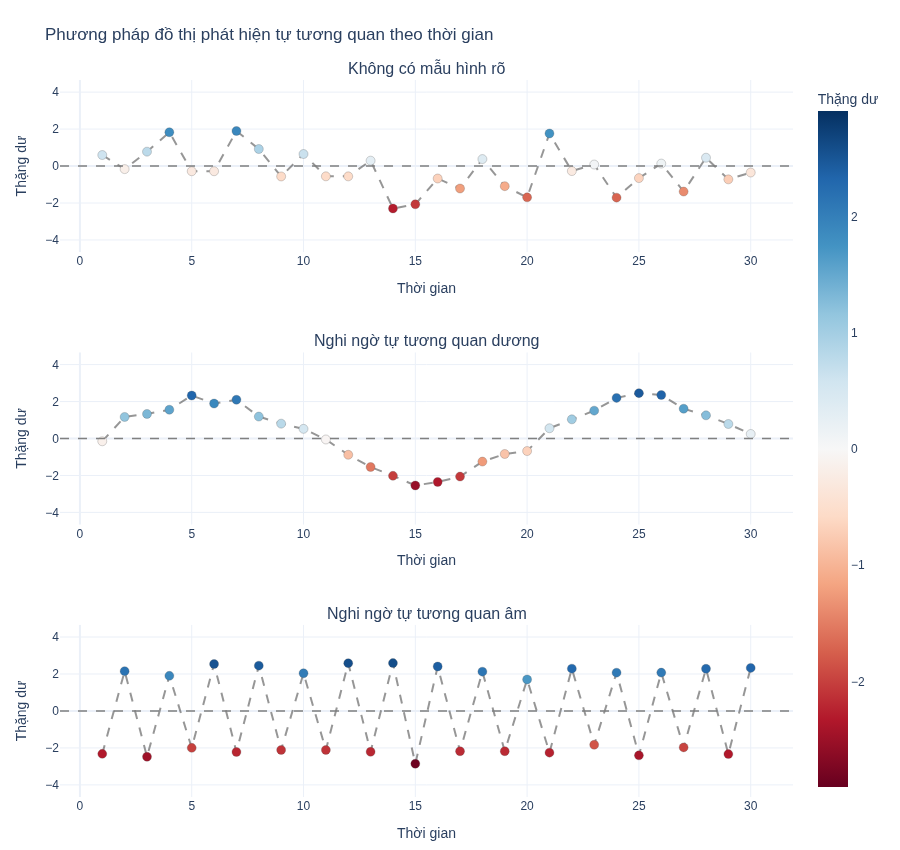
\includegraphics[width=\textwidth]{./media/plot_ts.png}
  \caption{Minh họa phần dư theo thời gian. Các cụm phần dư cùng dấu hoặc mẫu hình lặp lại là tín hiệu ban đầu của tự tương quan.}
  \label{fig:autocorr_time_residuals}
\end{figure}

\subsubsection{Phần Dư Theo Vị Trí hoặc Khu Vực}

Với dữ liệu không gian, có thể biểu diễn phần dư theo bản đồ, vị trí địa lý hoặc nhóm khu vực. Nếu các quan sát gần nhau có phần dư tương tự nhau, ví dụ cùng dương hoặc cùng âm, ta nghi ngờ tự tương quan theo không gian.

\begin{figure}[H]
  \centering
  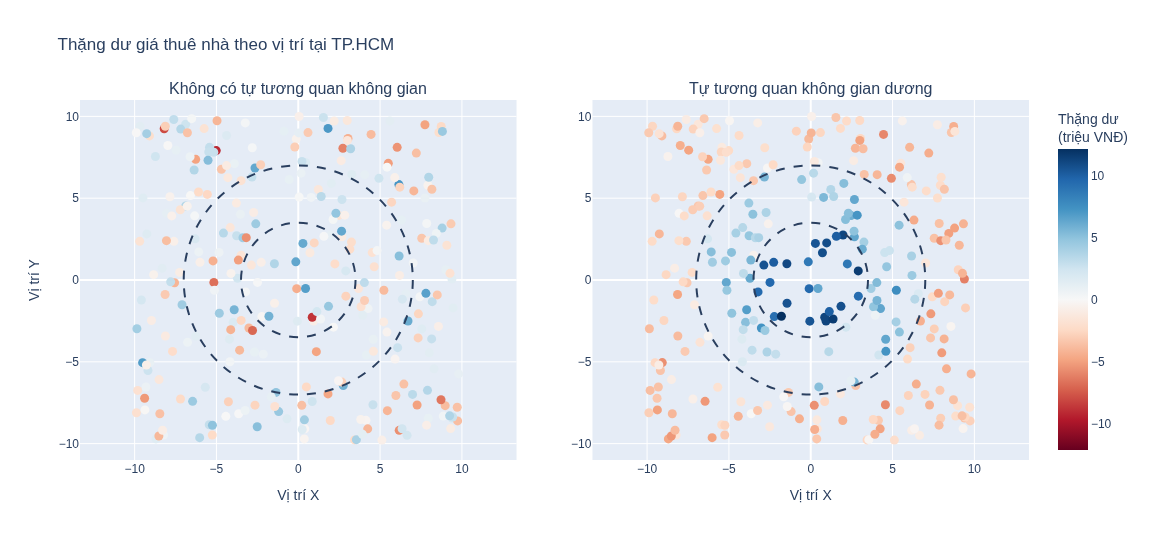
\includegraphics[width=\textwidth]{./media/rent_house.png}
  \caption{Minh họa tự tương quan theo không gian trong bài toán giá thuê nhà. Các cụm khu vực có phần dư tương tự nhau cho thấy mô hình có thể đang bỏ sót yếu tố vị trí.}
  \label{fig:autocorr_spatial_residuals}
\end{figure}

Phương pháp đồ thị giúp nhận diện mẫu hình ban đầu nhưng vẫn có yếu tố chủ quan. Vì vậy, kết luận chính thức nên kết hợp thêm kiểm định thống kê phù hợp với loại dữ liệu.

% -----------------------------------------------------------------------------
